\documentclass{beamer}
\usetheme[white]{Wisconsin}
\usepackage{longtable}
\usepackage{listings}
\usepackage{color}
%% The amssymb package provides various useful mathematical symbols
\usepackage{amssymb}
%% The amsthm package provides extended theorem environments
\usepackage{amsthm} \usepackage{amsmath} \usepackage{tmadd,tmath}
\usepackage[mathcal]{euscript} \usepackage{color}
\usepackage{textcomp}
\usepackage{algorithm,algorithmic}
\definecolor{listinggray}{gray}{0.9}
\definecolor{lbcolor}{rgb}{0.9,0.9,0.9}
\lstset{
  backgroundcolor=\color{lbcolor},
  tabsize=4,
  rulecolor=,
  language=c++,
  basicstyle=\scriptsize,
  upquote=true,
  aboveskip={1.5\baselineskip},
  columns=fixed,
  showstringspaces=false,
  extendedchars=true,
  breaklines=true,
  prebreak =
  \raisebox{0ex}[0ex][0ex]{\ensuremath{\hookleftarrow}},
  frame=single,
  showtabs=false,
  showspaces=false,
  showstringspaces=false,
  identifierstyle=\ttfamily,
  keywordstyle=\color[rgb]{0,0,1},
  commentstyle=\color[rgb]{0.133,0.545,0.133},
  stringstyle=\color[rgb]{0.627,0.126,0.941},
}

%% colors
\setbeamercolor{boxheadcolor}{fg=white,bg=UWRed}
\setbeamercolor{boxbodycolor}{fg=black,bg=white}


%%---------------------------------------------------------------------------%%
\author{Stuart R. Slattery
  \\ Engineering Physics Department
  \\ University of Wisconsin - Madison
}

\date{\today} 
\title{$SP_N$ Update} 
\begin{document}
\maketitle

%%---------------------------------------------------------------------------%%
\begin{frame}{Neutron Transport Solution Methods}

  \begin{multline}
    \hat{\Omega} \cdot \vec{\nabla} \psi(\vec{r},\hat{\Omega},E) +
    \sigma(\vec{r},E) \psi(\vec{r},\hat{\Omega},E) = \\ \int \int
    \sigma_s(\vec{r},E' \rightarrow E,\hat{\Omega}' \rightarrow
    \hat{\Omega}) \psi(\vec{r},\hat{\Omega}',E') d\Omega' dE' +
    q(\vec{r},\hat{\Omega},E)
    \label{eq:general_transport}
  \end{multline}

  \begin{itemize}
  \item $S_N$ transport is expensive
    \begin{itemize}
    \item Difficult to parallelize: sweeps in space, pipelining in
      angle, energy decoupling
    \item Large storage requirements
    \item Ray effects
    \end{itemize}
  \item $P_N$ equations still expensive
    \begin{itemize}
    \item Complicated system: $(N+1)^2$ equations in 3D
    \item Coupling of equations through both angular moments and
      spatial derivatives
    \end{itemize}
  \end{itemize}
\end{frame}

%%---------------------------------------------------------------------------%%
\begin{frame}{$SP_N$ Approximation}
  \begin{itemize}
  \item Ad-hoc generalization of planar $P_N$ equations by Gelbard in
    the 1960's
  \item Rigorous formulation through asymptotic and variational
    analysis in 1990's and 2000's
  \item Simpler system $(N+1)/2$ equations in $3D$
  \item Yields elliptic, diffusion-like equations
  \item Applicable when diffusion theory is applicable: reasonable
    flux gradients, full-core transport
  \item Typically does not converge to transport solution as
    $N\rightarrow \infty$
  \item {\bf Can build the full linear operator}
  \item {\bf Parallelism through the linear solver}
  \end{itemize}
\end{frame}

%%---------------------------------------------------------------------------%%
\begin{frame}{$SP_N$ Approximation}

  \begin{beamerboxesrounded}[upper=boxheadcolor,lower=boxbodycolor,shadow=true]
    {$SP_N$ Equations}
    \begin{multline}
      -\nabla \cdot \Bigg[\frac{n}{2n+1}\frac{1}{\Sigma_{n-1}} \nabla
        \Big(\frac{n-1}{2n-1} \phi_{n-2} + \frac{n}{2n-1}\phi_n \Big)
        \\+ \frac{n+1}{2n+1}\frac{1}{\Sigma_{n+1}} \nabla
        \Big(\frac{n+1}{2n+3}\phi_n + \frac{n+2}{2n+3}\phi_{n+2}\Big)
        \Bigg] \\+ \Sigma_n \phi_n = q \delta_{n0}\ \ \ \ \ \ \ \ \ n
      = 0,2,4,\cdots,N\:,
      \label{eq:spn_equations}
    \end{multline}
  \end{beamerboxesrounded}

\end{frame}

%%---------------------------------------------------------------------------%%
\begin{frame}{$SP_N$ Numerical Spectral Analysis}

  \begin{itemize}
    \item Monte Carlo methods for have strong restrictions on the
      eigenvalues of the operator for convergence
    \item MCSA has the same restrictions on the outer stationary
      iteration
    \item We need to compute these eigenvalues for various forms of
      the $SP_N$ equations to verify convergence of these methods.
  \end{itemize}

  We need eigenvalues for $\mathbf{A}$, $\mathbf{H_{J}}$, and
  $\mathbf{H_{GS}}$ with:
  \begin{equation}
    \mathbf{H_{J}} = \mathbf{I} - \mathbf{D}^{-1} \mathbf{A}
    \label{eq:jacobi_iteration_matrix}
  \end{equation}
  where $\mathbf{D} = diag(\mathbf{A})$ and 
  \begin{equation}
    \mathbf{H_{GS}} = (\mathbf{L+D})^{-1}\mathbf{U}
    \label{eq:gauss_seidel_iteration_matrix}
  \end{equation}

\end{frame}

%%---------------------------------------------------------------------------%%
\begin{frame}{$SP_7$, $P_3$, 3 groups, reflecting boundaries}

  \begin{columns}

    \begin{column}{0.5\textwidth}
      \begin{figure}[h!]
        \centering
        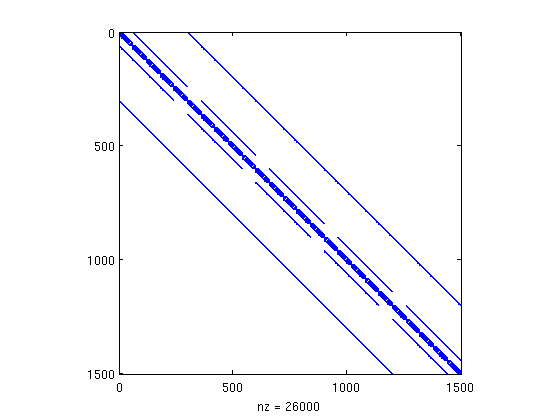
\includegraphics[width=2.5in,clip]{opSpySPn7P3G3.png}
        \caption{\textbf{Linear operator sparsity pattern}}
      \end{figure}
    \end{column}

    \begin{column}{0.5\textwidth}
      \begin{figure}[h!]
        \centering
        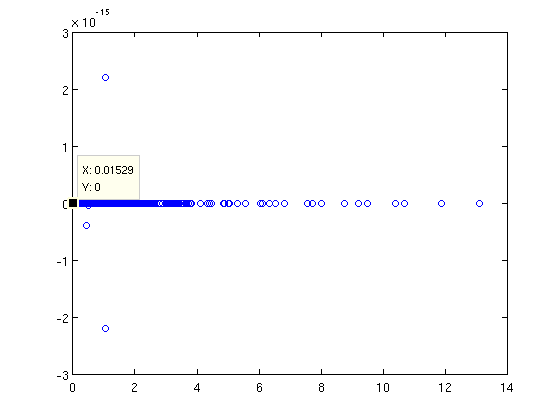
\includegraphics[width=2.5in,clip]{opSPn7P3G3.png}
        \caption{\textbf{Linear operator eigenvalues}}
      \end{figure}
    \end{column}

  \end{columns}

\end{frame}

%%---------------------------------------------------------------------------%%
\begin{frame}{$SP_7$, $P_3$, 3 groups, reflecting boundaries}

  \begin{columns}

    \begin{column}{0.5\textwidth}
      \begin{figure}[h!]
        \centering
        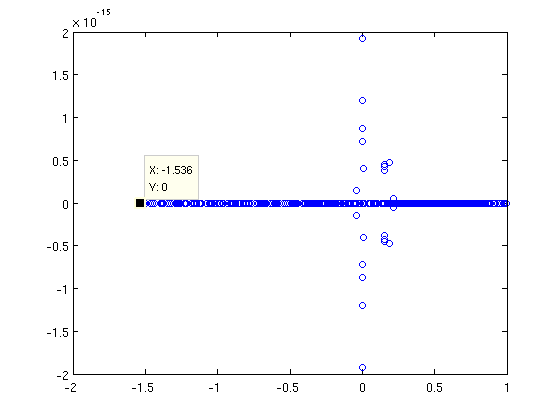
\includegraphics[width=2.5in,clip]{SPn7P3G3.png}
        \caption{\textbf{Jacobi iteration matrix eigenvalues}}
      \end{figure}
    \end{column}

    \begin{column}{0.5\textwidth}
      \begin{figure}[h!]
        \centering
        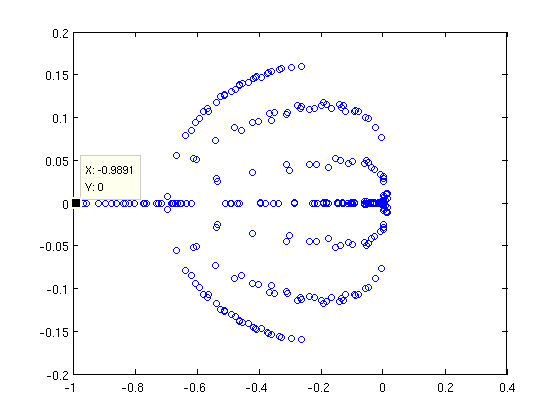
\includegraphics[width=2.5in,clip]{gsSPn7P3G3.png}
        \caption{\textbf{Gauss-Seidel iteration matrix eigenvalues}}
      \end{figure}
    \end{column}

  \end{columns}

\end{frame}

%%---------------------------------------------------------------------------%%
\begin{frame}{Oh No!}

  \begin{itemize}
    \item The Jacobi method won't converge - all that stuff I said in
      my prelim won't work
  \end{itemize}

\end{frame}

%%---------------------------------------------------------------------------%%
\begin{frame}{Solution}

  \begin{itemize}
  \item Bug fix in Denovo $SP_N$ implementation
  \item A new kind of preconditioning $\cdots$
  \end{itemize}

\end{frame}

%%---------------------------------------------------------------------------%%
\begin{frame}{Multigroup Matrix Pattern}

  \begin{figure}[h!]
    \centering
    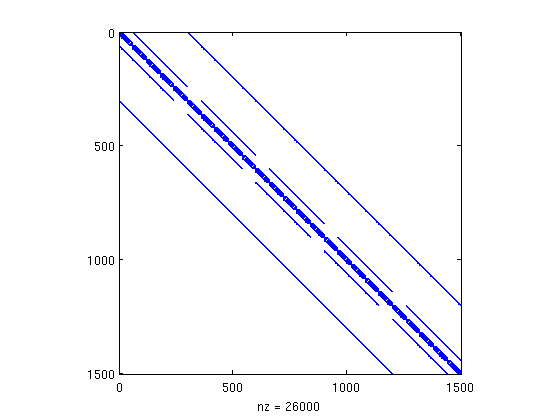
\includegraphics[width=2.5in,clip]{opSpySPn7P3G3.png}
    \caption{\textbf{Linear operator sparsity pattern}}
  \end{figure}

\end{frame}

%%---------------------------------------------------------------------------%%
\begin{frame}{Block Jacobi Preconditioning}

  \begin{figure}[h!]
    \centering
    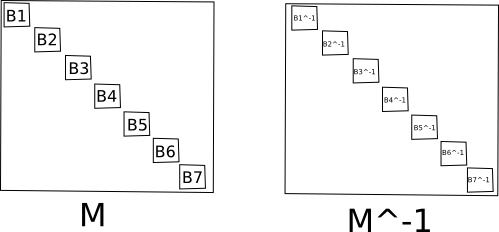
\includegraphics[width=4in,clip]{block_preconditioning.png}
    \caption{\textbf{Block Jacobi Preconditioner}}
  \end{figure}

\end{frame}

%%---------------------------------------------------------------------------%%
\begin{frame}{Point Jacobi Results}

  \begin{figure}[h!]
    \centering
    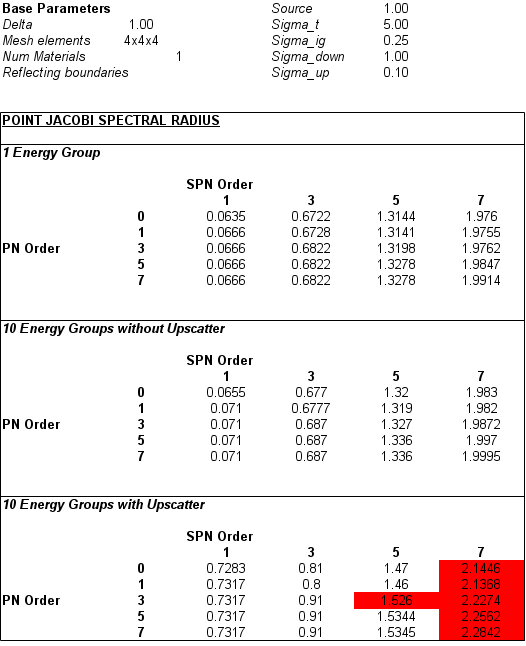
\includegraphics[width=2.5in,clip]{point_jacobi_data.png}
    \caption{\textbf{Point Jacobi Preconditioning for $SP_N$ Equations}}
  \end{figure}
  
\end{frame}

%%---------------------------------------------------------------------------%%
\begin{frame}{Block Jacobi Results}

  \begin{figure}[h!]
    \centering
    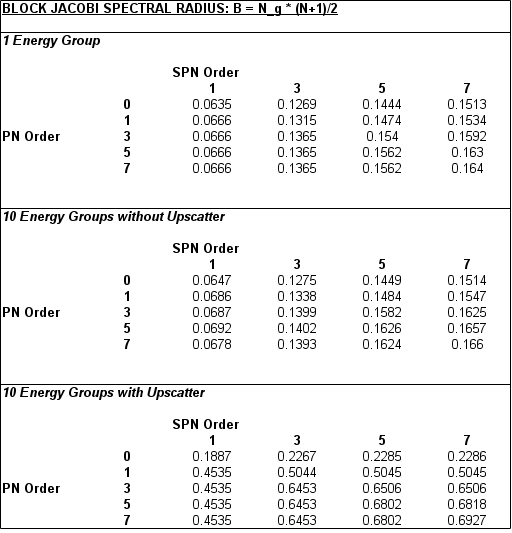
\includegraphics[width=3in,clip]{block_jacobi_data.png}
    \caption{\textbf{Block Jacobi Preconditioning for $SP_N$ Equations}}
  \end{figure}
  
\end{frame}

%%---------------------------------------------------------------------------%%
\begin{frame}{Conclusions}

  \begin{itemize}
  \item Block Jacobi preconditioning is a simple and appropriate
    solution for preconditioning the $SP_N$ equations
  \item Implementation is general - slides right into ANA framework
  \item Implementation is scalable - local operations only, fast
    LAPACK operations
  \item Implementation works - can move on with research
  \end{itemize}

\end{frame}

%%---------------------------------------------------------------------------%%

\end{document}
